\documentclass[12pt,fleqn]{article}
\setlength{\parindent}{0pt}
\usepackage{graphicx}
\usepackage{listings}
\usepackage[latin5]{inputenc}
\setlength{\parskip}{8pt}
\setlength{\parsep}{0pt}
\setlength{\headsep}{0pt}
\setlength{\topskip}{0pt}
\setlength{\topmargin}{0pt}
\setlength{\topsep}{0pt}
\setlength{\partopsep}{0pt}
\setlength{\mathindent}{0cm}

\begin{document}
MIT OCW Cok Degiskenli Calculus - Ders 9

Bu dersin konusu birden fazla degisken iceren fonksiyonlarin minimizasyonu
ile ugrasirken yardimci olacak kismi turev (partial derivative)
kavrami. Cok degiskenli bir fonksiyon $f(x,y)$'nin birden fazla turevi
vardir. Mesela bunlardan bir tanesi

\[ \frac{\partial f}{\partial x} = f_x \]

Bu turev $x$'in degistirildigi ama $y$'nin sabit tutuldugu bir durumu
gosterir. 

\[ \frac{\partial f}{\partial y} = f_y \]

ise $y$'in degistirildigi ama $x$'nin sabit tutuldugu bir durumu gosterir.

Simdi her ikisinin birden degistirildigi durumda ne olacagini gosteren
yaklasiksal (approximate) formulu gorelim. Degisim matematiksel olarak
soyle

\[ x \sim x + \Delta x \]

\[ y \sim x + \Delta x \]

O zaman $z$ icin

\[ z = f(x,y) \]

yaklasiksal degisim soyle olur

\begin{equation}\label{eq1}
\Delta z \approx f_x\Delta x + f_y \Delta f_y
\end{equation}


Tekrar vurgulamak gerekirse bu yaklasiksal bir formul, daha ``dogru'' bir
temsil icin 2., 3. turevleri iceren daha yuksek dereden (higher order
terms) terimlerin de olmasi gerekir, fakat bu terimler 1. derece lineer bir
yaklasiksallik icin kullanilmaz. 

Bu formulu nasil dogrulariz? Bunu yapmanin yollarindan biri teget duzlem
yaklasiksallamasi (tangent plane approximation). Mesela $z = f(x,y)$
fonksiyonuna olan teget bir duzlemi dusunelim.

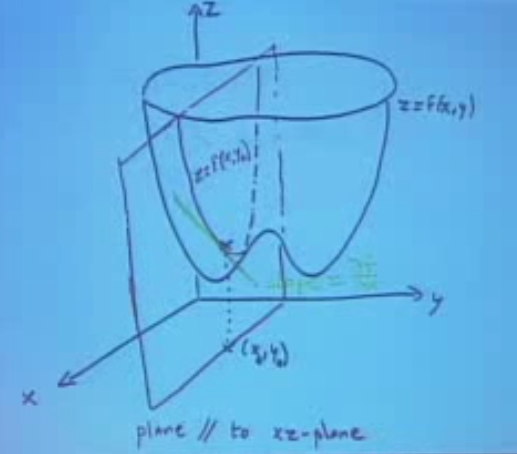
\includegraphics[height=4cm]{9_1.png}

Hatirlarsak $\frac{\partial f}{\partial x}$ kismi turevi $x$'in degistigi
ama $y$'nin sabit tutuldugu bir durumu tarif ediyordu. Yukaridaki grafige
gore bu bir anlamda iki cukurlu kap gibi duran $z$ fonksiyonun bir kesitine
bakmak gibi (unutmayalim, fonksiyon sadece kabin disinda tanimli, ici
bos). Bu kesit $f$'in bir yansimasini olusturuyor, o yansima ustteki
grafikte bir parabol seklinde. Bu parabolda $x$ degistikce o noktanin
parabol uzerindeki cizgizel tegeti de degisiyor (grafikteki yesil cizgi) ki
bu cizgisel egim $\frac{\partial f}{\partial x}$'e esit. 

Eger ayni seyi $x$'in sabit $y$'nin sabit oldugu durum icin yapsaydim,
benzer bir kesit elde edecektim. 

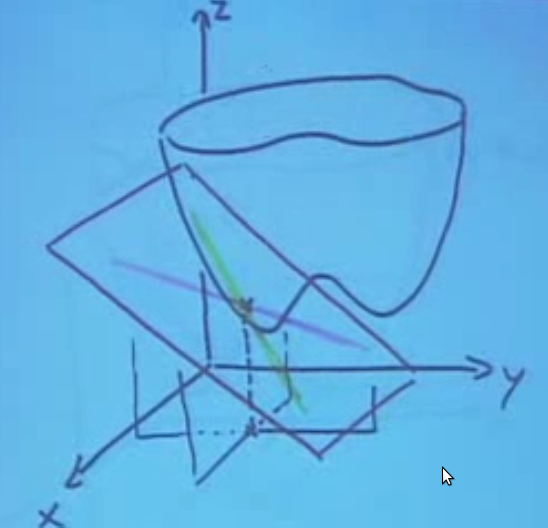
\includegraphics[height=4cm]{9_2.png}

Bu iki kesit uzerinden elde edilen ikinci teget cizgi birinci ile beraber
kullanilinca bir duzlemi tanimlamak icin kullanilabilir (iki cizgi paralel
bir duzlem tanimlamak icin yeterlidir), ki teget duzlem yaklasiksallamasi
icin kullanilacak duzlem budur. Bunu nasil yapacagimizi gosterelim.

$f_x$ ve $f_y$ iki teget cizgiyi tanimlamak icin kullaniliyorsa, bu
formulleri bir araya koyarak duzlemi temsil edebilirim. Eger

\[ \frac{\partial f}{\partial x}(x_0,y_0) = a \]

ise bu demektir ki birinci teget cizgi (yesil cizgi) $L_1$ soyledir:

\[ 
L_1 = 
\left\{ \begin{array}{l}
z = z_0 + a(x - x_0) \\
y = y_0
\end{array} \right.
 \]

Bu cizgi icin $y$'yi sabit tutuyorum, $z$'deki degisimi $z_0$ ustune egim
$a$'nin katlari kadar ($x$'in degisimi oraninda carparak) ekleyerek
hesapliyorum. 

Benzer sekilde

\[ \frac{\partial f}{\partial y}(x_0,y_0) = b \]

\[ 
L_2 = 
\left\{ \begin{array}{l}
z = z_0 + b(y - y_0) \\
y = y_0
\end{array} \right.
 \]

Hem $L_1$ hem de $L_2$ $z = f(x,y)$'ye tegettir. Bu iki cizgi beraber bir
duzlem olusturur. Bu formul

\begin{equation}\label{eq2}
z = z_0 + a(x-x_0) + b(y-y_0) 
\end{equation}

formuludur. 

Formul \ref{eq1}, ustteki formulun yaklasiksal halidir. Eger teget duzlem
uzerinde olsaydik, $\approx$ isareti $=$ isaretine donusecekti. Bu
yaklasiksallik ufak $\Delta x$ ve ufak $\Delta y$ icin gecerli. Yani
yaklasiksal formul, $f$'nin grafigi teget duzleme yakin diyor. 

Maksimum Minimum Problemleri 

Kismi turevlerin kullanim alanlarindan biri optimizasyon
problemleridir. Mesela cok degiskenli bir fonksiyonun maksimumunu bulmak
gibi. Eger fonksiyon tek degiskenli olsaydi, hemen turevini alip sonucu
sifira esitleyebilirdik, ve buna gore bir cozum arardik. Cok degiskenli
fonksiyonlarda kismi turevler kullanmak lazim. 

Bu derste iki degiskenli duruma bakacagiz fakat ayni prensipler, 10, 15,
milyon tane degisken icin ayni. 

Lokal bir minimum icin hem $f_x=0$ hem $f_y=0$ olmalidir. Bu niye
dogudur. Yine formul \ref{eq1}'e bakarsak, hem $f_x=0$ hem $f_y=0$ oldugu
zaman $\Delta z$ sifir olacaktir, yani birinci derecede dusunursek
$f(x,y)$'de degisim yok demektir. 

Teget duzlemlerin dilinden konusursak, minimum aninda teget duzlem tamamen
yatay olacaktir. 

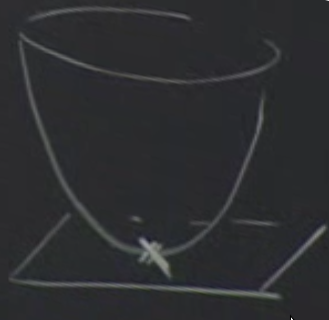
\includegraphics[height=3cm]{9_3.png}

Formul \ref{eq2} baglaminda dusunursek, bu durum $a=0$ ve $b=0$ oldugu ana
tekabul ediyor ve o anda duzlemi tanimlayan $z = z_0$ formuludur. 

Tanim

Eger $f_x(x_0,y_0)= 0$ ve $f_y(x_0,y_0)= 0$ ise o zaman $x_0,y_o$ $f$'in
kritik noktasidir. Not: Birden fazla degisken icin tabii ki tum kismi
turevlerin o noktada sifir olmasi gerekir.

Ornek

\[ f(x,y) = x^2 - 2xy + 3y^2 + 2x - 2y \]

Bakalim bunu minimize ya da maksimize edebilecek miyiz? 

\[ f_x = 2x - 2y + 2 = 0\]

\[ f_y = -2x + 6y - 2 = 0 \]

Ustteki iki denklemi ayni anda cozmeliyiz. 

Bu tur durumlarda iki denklemi birbiriyle toplayip basitlestirmeye calismak
iyi bir yontemdir. Fakat unutmayin, elimizde her zaman iki tane denklem
olmali, iki denklemi ortadan kaldirip birdenbire tek denklem ile yola devam
edemeyiz. 

Toplami yaparsak

\[ 4y = 0 \]

elde ederiz. Bunu alip birinci denkleme sokalim, sonuc

\[ 2x + 2 = 0 \]

\[ x = -1 \]

Demek ki kritik nokta $(x,y) = (-1,0)$. 

Peki bu kritik noktanin minimum mu maksimum mu oldugunu nereden bilecegiz?
Eger tek degiskenli bir fonksiyona bakiyor olsaydik, ikinci tureve
bakabilirdik. Benzer bir seyi burada da yapabilirdik, ama sadece birinci
turevden bile elimizde iki tane var, ikinci turevlerden cok daha fazlasi
olacak. O duruma bakacagiz, simdilik daha az otomatik olarak isi nasil
anlayacagimizla ilgilenelim. 

Elimizde birden fazla minimum olabilir. Turev(lerin) sifir oldugu noktada
bir duzluk vardir, bu bir lokal minimumdur. Yani o noktaya yakin oldugumuz
surece (ki lokalligin tanimi bu) bu minimum gecerlidir. Baska bir noktada,
turev(lerin) yine sifir oldugu ama daha asagi noktada bir minimum daha
olabilirdi. Maksimumlar icin ayni durum gecerli.

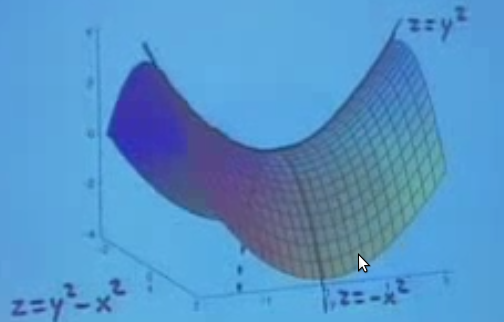
\includegraphics[height=4cm]{9_4.png}

Yanliz bir diger secenek daha var. Bu secenek kritik noktanin ne maksimum,
ne minimum oldugu durumdur. Bu durumda kritik noktadan hangi ``yone dogru''
bakiyorsak, degisik bir cevap elde ederiz. Bu at egeri gibi gozuken
grafigin orta noktasina, 0,0,0 noktasina bakalim, burada teget duzlem tam
yatay. Bu noktaya eger noktasi (saddle point) deniyor. 

2. turevlerden bahsetmisik, ve bu derste kritik noktanin ne oldugunu daha
az otomatik bulacagimizi soyledik (2. turevler bir dahaki derste). 

Bu yontemde kareler kullanacagiz. $f(x,y)$'nin kareler, ve onlarin toplami
olduguna dikkat edelim. Eger tum formulu bir seyin karesi olarak
gosterebilirsek, belki bir yerlere gelebiliriz. Tek problem $xy$ terimi,
ama $x^2 - 2x..$ diye giden bir formul biliyoruz. Kareyi Tamamlama
teknigini kullanabiliriz. 

\[ f(x,y) = (x-y)^2 + 2y^2 + 2x - 2y \]

Basitlesti ama biraz daha basitlesebilir. Acaba $(x-y)^2$ icindeki $(x-y)$
ile disaridaki $2x - 2y$ arasindaki bir baglanti kurabilir miyim? Iceriye
bir +1 eklersek bu olabilir. O zamam disaridaki $2x - 2y$ iptal
olur. Icerideki 1'i dengelemek icin disari bir -1 ekleriz. 

\[  = ((x-y) + 1)^2 + 2y^2 - 1\]

Bu formul eger 

\[  = \underbrace{((x-y) + 1)^2}_{\ge 0} + \underbrace{2y^2}_{\ge 0} - 1\]

ise ancak $\ge -1$ olabilir. Ve kritik nokta (-1,0)[da $f$'in degeri
hakikaten -1'dir. Niye ustteki iki terim $\ge 0$ dedik? Cunku bu terimler
karesel ifadeler, ve karesel ifadeler en az sifir olabilirler. Bir deger ne
olursa olsun, eksi bile olsa karesi alinirsa artik olur, bu tur ifadeler
sadece sifirda ``en az'' olurlar. Yani biraz cebirsel takla, ve ufak bir
numarayla istedigimiz sonuca erismis olduk.





\end{document}
